\documentclass[a4paper]{article}

%% Language and font encodings
\usepackage[english]{babel}
\usepackage[utf8x]{inputenc}
\usepackage[T1]{fontenc}

%% Sets page size and margins
\usepackage[a4paper,top=3cm,bottom=2cm,left=3cm,right=3cm,marginparwidth=1.75cm]{geometry}

%% Useful packages
\usepackage{amsmath}
\usepackage{graphicx}
\usepackage{luacode} % <-- Necessary for CSV tables!
\usepackage[colorinlistoftodos]{todonotes}
\usepackage[colorlinks=true, allcolors=blue]{hyperref}

\title{overleaf-stata-demo}
\author{Benjamin B. Daniels}

\begin{document}
\maketitle

\section{Figures and tables with overleaf-stata-tools}

The overleaf-stata-tools repo (https://github.com/bbdaniels/overleaf-stata-tools) contains several utilities for using Overleaf as a dynamic documents processor. For a full demo, clone https://git.overleaf.com/15274949kphkgfxjmhxb (this Overleaf project) to desktop to observe the file structure and the LuaLaTeX implementation of CSV tables in action. The repo contains:

\begin{enumerate}
\item {\it gitSuite}, a wrapper for three Git shell commands:
	\begin{enumerate}
	\item {\it gitReady}, which checks installations and sets a \${git} global pointing to your Overleaf local clone
    \item {\it gitSet}, which pulls the Overleaf remote before creating outputs to ensure there are no conflicts
    \item {\it gitGo}, which pushes the Overleaf local to remote once creation of outputs is complete
    \end{enumerate}
\item {\it mat2csv}, which takes an arbitrary Stata matrix with NAME (and, optionally, an identically-sized matrix called NAME\_STARS) and writes a well-formatted CSV
	\begin{enumerate}
	\item This CSV can be read by Caleb Reister's csv.lua script for immediate translation into a TeX table. (https://github.com/calebreister/TeX-Utilities) This may require manually setting the engine to LuaLaTeX in Overleaf, and always requires \textbackslash usepackage\{luacode\}.
    \end{enumerate}
\item {\it reg2csv}, which takes an arbitrary set of Stata regressions in memory and produces a regression table with the estimates, standard errors, and estimation statistics in the above format.
	\begin{enumerate}
	\item Syntax and code base are substantially thanks to Michael Lokshin and Zurab Sajaia's excellent {\it xml\_tab} (http://ageconsearch.umn.edu/bitstream/122600/2/sjart\_dm0037.pdf).
    \end{enumerate}
    
\end{enumerate}


\begin{figure}
\centering
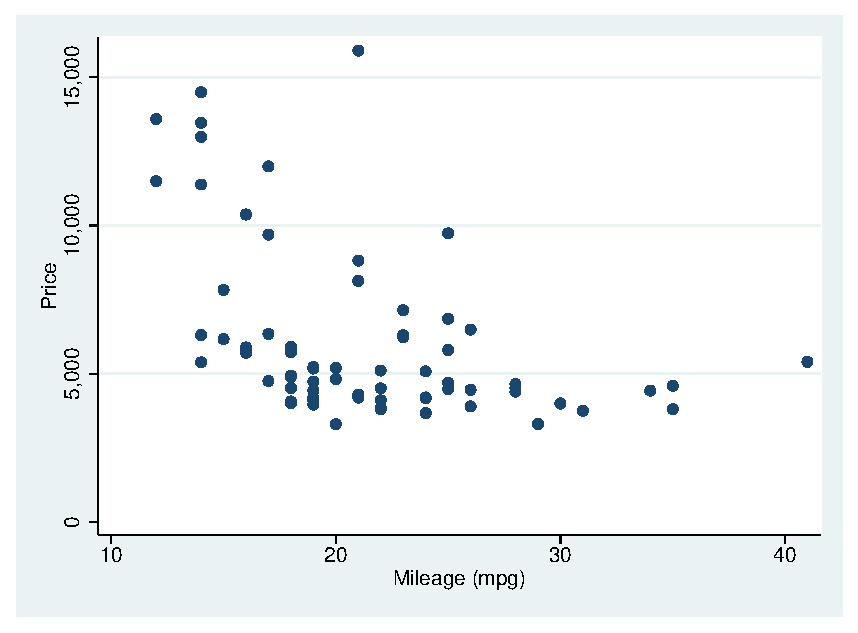
\includegraphics[width=1\textwidth]{figure.eps}
\caption{\label{fig:figure}Demo figure}
\end{figure}

\begin{table}
\centering
\begin{tabular}{lrrrrrrr}
  \hline
  \luaexec{
    require('csv.lua')
    t = dataToTable('test.csv')
    tex.sprint(tableToTeX(t, '\\hline',{2}))
    } \\
  \hline
  \end{tabular}
\end{table}

\begin{table}
\centering
\begin{tabular}{l|rrrrrrr}
  \hline
  \luaexec{
    require('csv.lua')
    t = dataToTable('regtest.csv')
    tex.sprint(tableToTeX(t, '\\hline',{2,10}))
    } \\
  \hline
  \end{tabular}
\end{table}

\end{document}